\section{Introduction}
In unserer Welt verlassen wir uns darauf, dass Dinge (in unserem Fall Programme) funktionieren. Aber alles kann kaputt gehen, meistens wenn wir es am wenigsten erwarten. Vor allem in der Bemannten Raumfahrt können Fehler zu verheerenden Katastrophen führen.

\subsection*{Introduction to Fault Tolerance}
Patterns for Fault Tolarant Software versucht mögliche Lösungen aufzuzeigen wie auf das Auftreten von Fehlern in Systemen reagiert werden kann. Und wie ein System noch lauffähig ist, auch wenn gewisse Teile ausgefallen sind oder nicht mehr korrekt funktionieren. Um aber über die Fehler Toleranz diskutieren zu können, müssen nachfolgenden Begriffe definiert werden.

\subsection{Fault, Error, Failure}
\begin{itemize}
	\item Failure (Ausfall): Ein System liefert nicht mehr die erwarteten Ergebnisse, da ein Fehler (Error) aufgetreten ist. Ausfälle können aber nur passieren, wenn definiert ist, was als korrektes Verhalten angesehen wird. Ist dies nicht spezifiziert, kann ein System auch nicht ausfallen.
	\item Error (Fehler): Der Zustand des Systems, wenn ein Defekt aufgetreten ist. Ein Fehler kann abgefangen werden, wenn er auftritt sodass ein Ausfall (Failure) vermieden werden kann.
	\item Fault (Defekt, Bug): Mögliche Ursache für das Auftreten eines Fehlers (Error). Bugs sind in jedem System vorhanden, werden aber erst erkannt, wenn sie zu einem Fehler (Error) führen.
\end{itemize}

\subsubsection*{Abhängigkeiten}
 Fault führt zu Error, Error kann Failure zur Folge haben.

\begin{figure}[H]
	\centering
	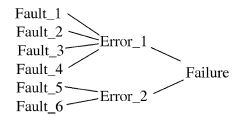
\includegraphics[width=8cm]{content/faulttolerance/images/fault-error-failure-dependency.jpg}
	\caption{Fault->Error->Failure Dependency}
\end{figure}

\subsubsection*{Failures}
 Bei fail-silent Failure wird entweder das korrekte Ergebnis zurückgegeben oder keines. So kann einfach entschieden werden, ob ein Ausfall Einfluss auf andere Systeme hat. Bei korrektem Ergebnis können alle Systeme gleich weiterarbeiten und falls kein Resultat vorliegt, ist der Ausfall eines Systems bekannt und kann entsprechend behandelt werden. Falls beim ersten Auftreten eines fail-silent Failures ein System nicht mehr weiterarbeitet, spricht man von einem crash Failure.

Grob kann man Ausfälle in zwei Gruppen einteilen:

\begin{itemize}
    \item Konsistent: gleiche Bedingungen führen zu gleichem Fehlverhalten, ist aber unabhängig vom Betrachter.
    \item Inkonsistent: Das Fehlverhalten ist abhängig vom Betrachter und von den Bedingungen, gleiche Bedingungen müssen aber nicht zu gleichem Fehlverhalten führen.
\end{itemize}

Fehlertolerantes Design versucht, inkonsistente Fehler in konsistente Fehler umzuwandeln, welche wiederum als fail-silent Failures behandelt werden können.

\begin{figure}[H]
	\centering
	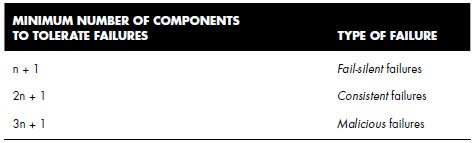
\includegraphics[width=\textwidth]{content/faulttolerance/images/failure-redundancy-num-components.jpg}
	\caption{Minimale Anzahl an Komponenten um Failures auszugleichen}
\end{figure}

\subsection{Coverage}
 Die Absicherung (Coverage) ist die Wahrscheinlichkeit, dass ein System in vorgegebener Zeit einen Fehler automatisch beheben kann.

\subsection{Reliability}

Die Zuverlässigkeit (Reliability) ist die Wahrscheinlichkeit, dass in einem System in vorgegebener Zeit keine Fehler auftreten.

\begin{itemize}
	\item \gls{MTTF} (Mean Time to Failure): Durchschnittliche Zeit vom Starten einer Operation bis zum ersten Ausfall.
	\item \gls{MTTR} (Mean Time to Repair): Durchschnittliche Zeit, die benötigt wird um eine ausgefallene Komponente wieder in einen funktionierenden Zustand zu versetzten.
	\item \gls{MTBF} (Mean Time between Failures): MTTF + MTTR
	\item \gls{FIT} (Failures in Time):  $\frac{Failures}{1e^{9}[h]}$
\end{itemize}

\textbf{Berechnung der Zuverlässigkeit:}
$reliability = e^{-(\frac{1}{\gls{MTTF}})}$

\subsection{Availability}
Die Verfügbarkeit (Availability) ist die Wahrscheinlichkeit in der Zeit, dass ein System erreichbar ist und seine vorgesehenen Aufgaben korrekt erledigen kann.

\begin{figure}[H]
	\centering
	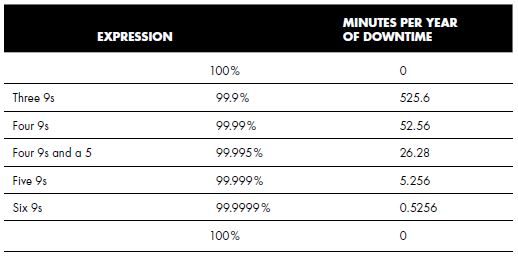
\includegraphics[width=\textwidth]{content/faulttolerance/images/downtime-per-year.jpg}
	\caption{Downtime per year}
\end{figure}

\textbf{Berechnung der Verfügbarkeit:}
$availability = \frac{\gls{MTTF}}{\gls{MTTF} + \gls{MTTR}}$

\subsection{Dependability}

Die Verlässlichkeit (Dependability) ist die Masseinheit für ein System wie stark man sich auf dessen Verlässlichkeit, Verfügbarkeit und Sicherheit verlassen kann. Die Sicherheit wird durch zwei Faktoren beeinflusst. Zu meinem der „Safety“ (Nichtauftreten von Ausfällen, die einen grösseren Schaden anrichten, als der Mehrwert, aller Vorteile eines System, mit sich bringt) und der „Security“ (Verhinderung von unautorisierten Zugriffen/Aktionen).

\subsection{Performance}

Die Leistungsfähigkeit (Performance) ist stark gekoppelt an die Zuverlässigkeit. Anforderungen an die Leistungsfähigkeit, können auch als Anforderungen an die Zuverlässigkeit gesehen werden und umgekehrt. Grundsätzlich kann festgehalten werden, dass Ausfälle, welche auf zu viele Anfragen zurückzuführen werden können, die Leistungsfähigkeit betreffen.

Falls dies geschieht, sind drei mögliche Szenarien möglich:

\begin{itemize}
	\item Crash: Das System bricht unter der Last zusammen
	\item Saturation: Das System läuft weiter, aber mit stark verminderter Leistungsfähigkeit (während der Überlastung) und kehrt schlussendlich wieder zu seiner erwarteten Leistungsfähigkeit zurück.
	\item Capacity decrease: Das System läuft weiter, aber die Leistungsfähigkeit wird dauerhaft vermindert bleiben.
\end{itemize}

\begin{figure}[H]
	\centering
	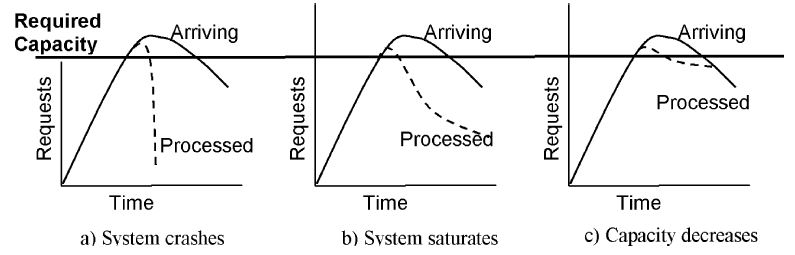
\includegraphics[width=\textwidth]{content/faulttolerance/images/performance.jpg}
	\caption{Performance}
\end{figure}